\Cref{fig:recent-program-margins} complements the event counts with the
recorded incumbent-utility difference for every promoted program.

\begin{figure*}[!tp]
  \setlength{\abovecaptionskip}{4pt}
  \centering
  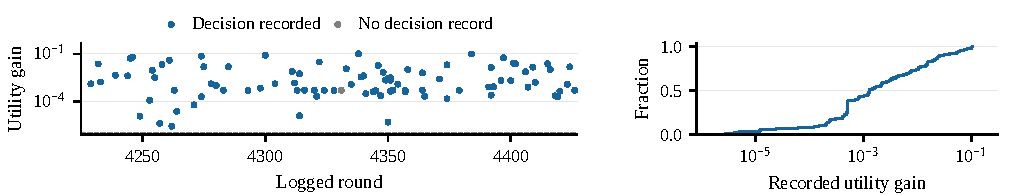
\includegraphics[width=\linewidth,height=1.25in,keepaspectratio]{figures/fig_recent_program_margins.pdf}
  \caption{\textbf{Recorded program gains span several orders of magnitude.}
  The same 92 two-fold training-program records as \cref{fig:program-round-counts},
  captured at 16:34 UTC on 3 November 2026. Left: each logged new utility
  minus its context's old incumbent utility, by round; grey retains the
  record at round 4331 with no decision record. The dashed line is the
  $10^{-6}$ promotion threshold. Right: the empirical cumulative distribution
  over all 92 differences. Gain axes are logarithmic; no records are clipped
  or smoothed. Positive gains are conditional on promotion, with no uncertainty
  intervals supplied; they do not establish adapter admission, writer learning
  or independent performance. Scope: \cref{sec:method-status}.}
  \label{fig:recent-program-margins}
\end{figure*}
